\chapter{Evaluation}
\label{ch:evaluation}
\section{Test drives}
Participants should be tested on the real road as simulators may allow testing for quantitative data, such as reaction time but hardly allows to recreate fear or discomfort ( \emph{\fullref{sec:studies}}). 

\subsection{Study Setup}
\label{sec:study}
In a counterbalanced, 2x2 experimental design setup, 
14 participants first rode either route A or route B, with the feedforward information (see \emph{\ref{ssec:feedforward}}) either turned on or off. Next, they rode in the inverse constellation (\emph{\fullref{tab:blocking}}). Test rides each had a total length of 45 minutes. 
The researcher welcomed participants in the lobby of the Bosch Technical Center in Plymouth and collected consent. Then subjects were on their own. They received a detailed instruction (\emph{\fullref{fig:instruction}}) and were positively 'primed'\footnote{\url{https://www.nngroup.com/articles/priming/}} about autonomous vehicles with a scenario.

\begin{quotation}
\begin{center} 
SCENARIO

Imagine that you do not own a car. Instead, you are calling an autonomous cab with an app on your smartphone whenever you need. 

There are multiple reasons why you chose not to own a car. Some of them are: hailing autonomous cabs is a cheaper alternative than owning a vehicle, driving yourself takes concentration and time, you get picked up and dropped off by the taxi wherever you want to, and moreover autonomous cars drive a lot safer than you could drive yourself. 

Today you take two rides in an autonomous vehicle. 
 \end{center}
\end{quotation}

\begin{figure}
     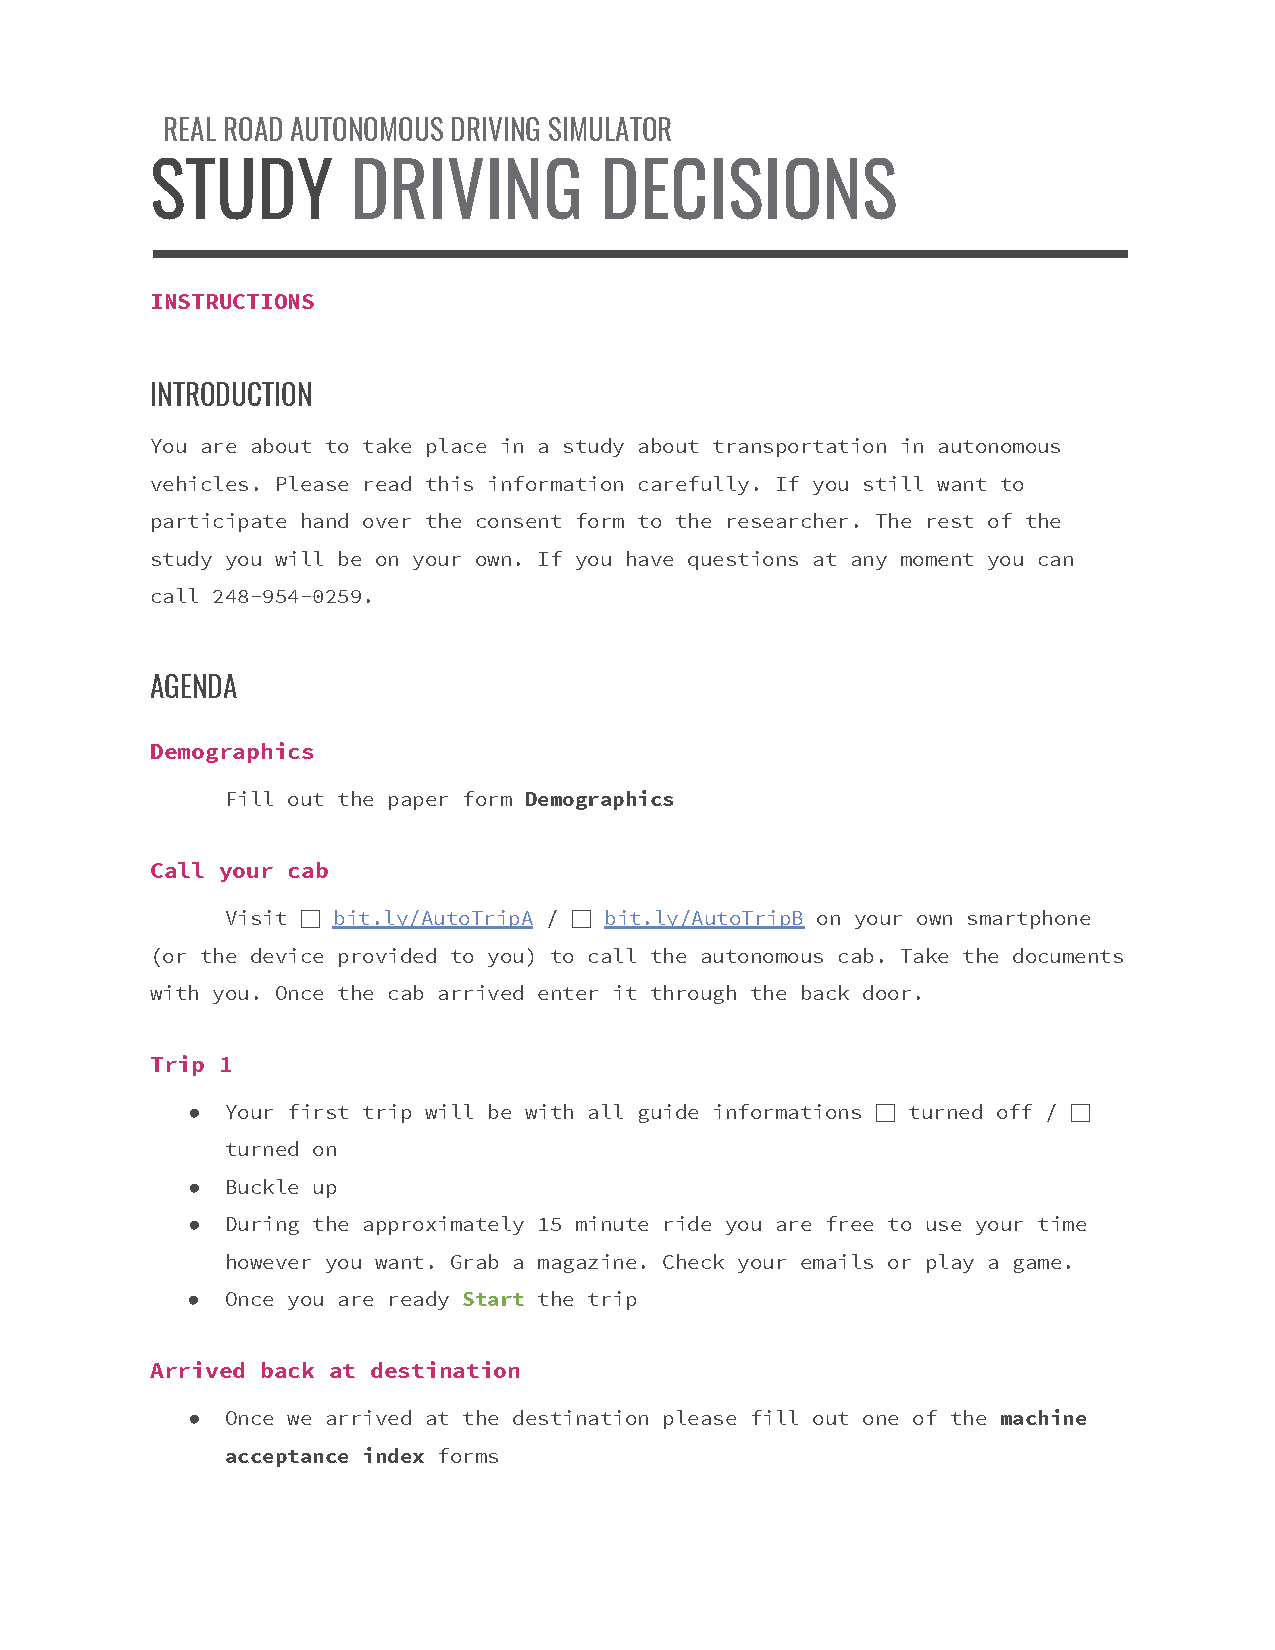
\includegraphics[width=0.5\textwidth]{fig/Instru1.pdf}\hfill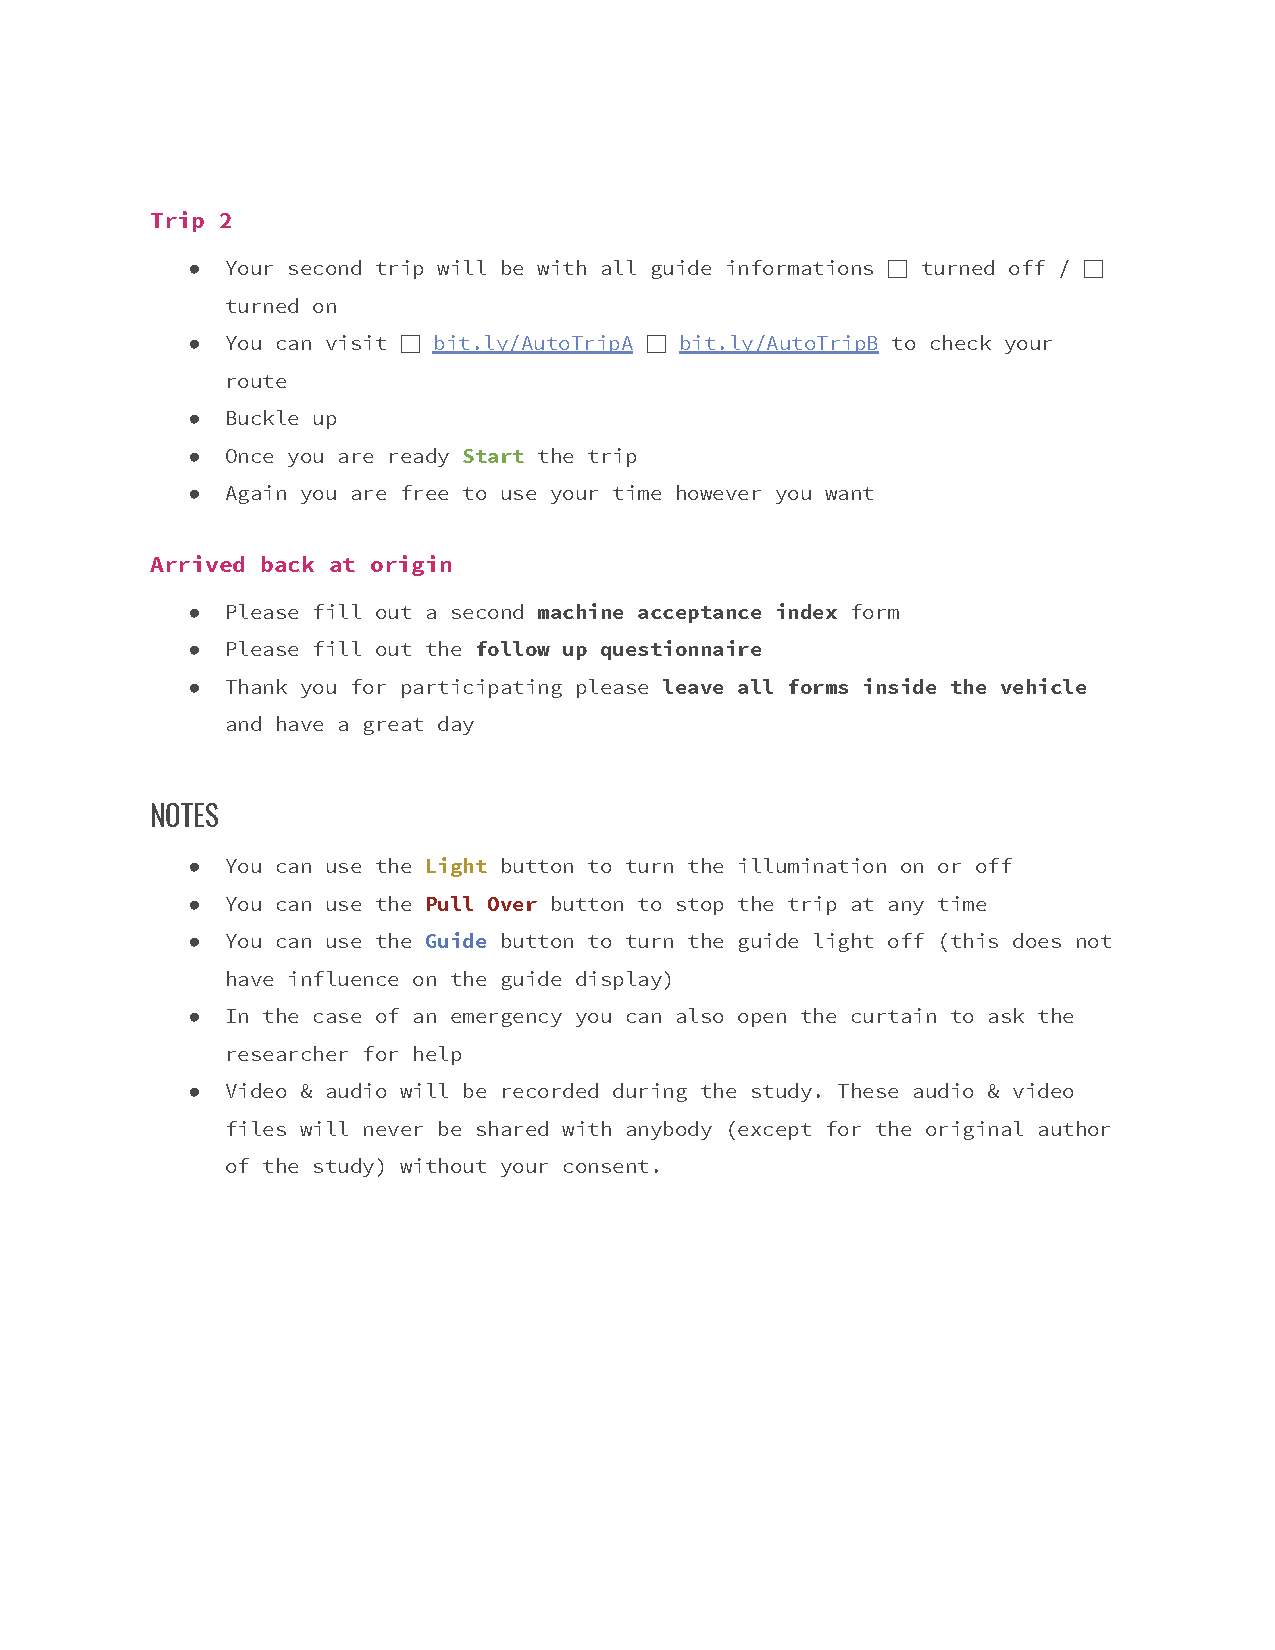
\includegraphics[width=0.5\textwidth]{fig/Instru2.pdf}
    \caption[Study Instruction]{Study instruction (Full resolution versions is attached in the digital appendix)}
    \label{fig:instruction}
\end{figure}

They called the cab with the web app (\emph{\fullref{sec:capp}}) as instructed. The cab arrived in front of the lobby and honked to inform of its arrival. Because of the angle, at which the vehicle approached and a curtain that separates passengers in the back from the wizards in front, participants could not establish eye contact. Once buckled up they pressed the 'start ride' button. 
\begin{figure}
     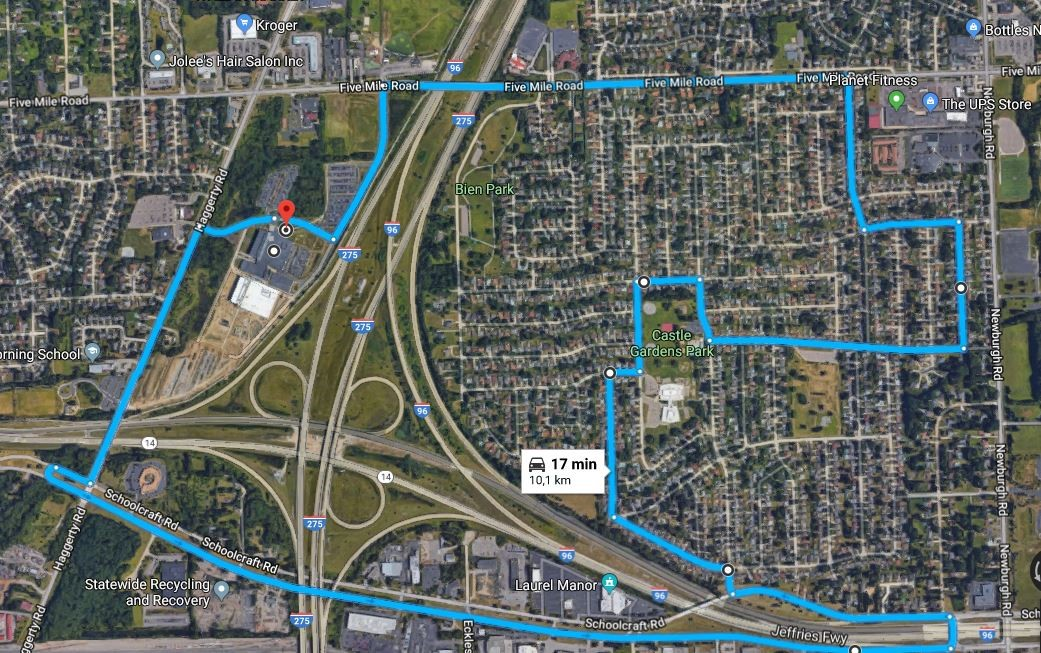
\includegraphics[width=\textwidth]{fig/RouteA_Mittel.JPG}\hfill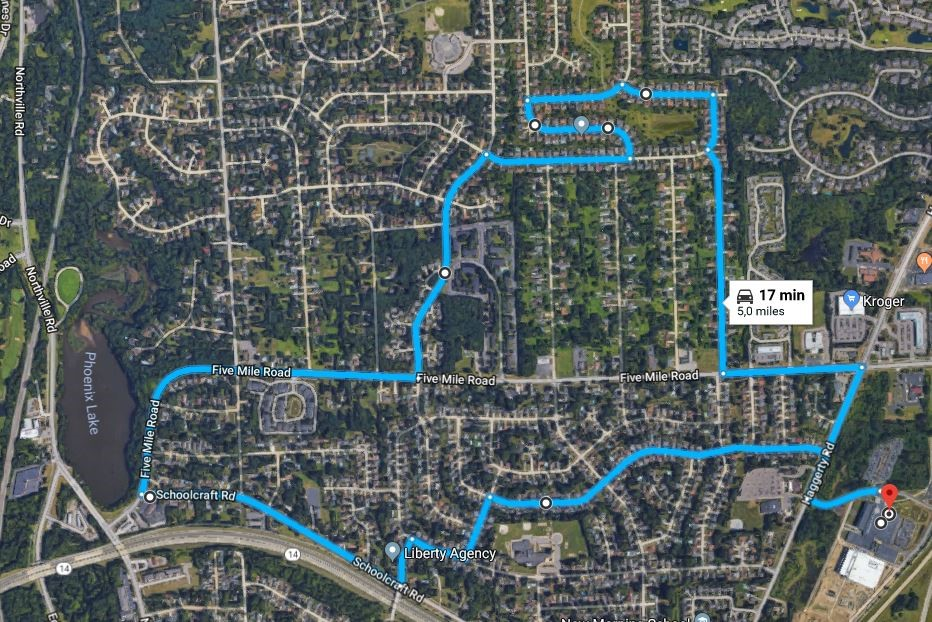
\includegraphics[width=\textwidth]{fig/RouteB_Mittel.JPG}
    \caption[Test routes]{Test routes. Top: Livonia (17min, 7.1km). Bottom: Northville (17min, 8.0km)}
    \label{fig:routes}
\end{figure}
The routes started and always ended at Bosch Technical Center in Plymouth. The tour through Northville was longer and had a higher top speed as parts of it used the highway (60mph). Both tours took approximately 17 minutes (\emph{\fullref{fig:routes}}). The tours differed so that participants did not have to drive the same route twice and did not pay less attention the second time (learning effects). 
During each of the rides, the subjects were videotaped and could use their time freely. The participants filled out one pre-study questionnaire, two of the same trust in automation questionnaires \citep{Jian2010,Koo2015} and a post-study questionnaire. In the feedforward-information-on (guide on) condition the cars decisions were augmented through the interaction wizard.

\begin{table}
  \caption{Blocking of study participants}
  \label{tab:blocking}

\begin{tabular}{@{}l|llll@{}}
\toprule
                    & First Livona & First Northville &  &  \\ \midrule
First without guide & 3+2          & 3                &  &  \\
First with guide    & 3            & 3                &  & 
\end{tabular}
\end{table}

\subsection{Vehicle}
For the on-the-road tests a red Nissan Cube test car (\emph{\fullref{fig:testsetup}}), which was acquired for software testing of an now in production infotainment system, was used. Even though the interior already came of age the outside reminds of a futuristic cab. The chassis of the vehicle drives a bit jerky (see \emph{\ref{ssec:interviews}}). Smoother acceleration and brake might influence the well-being of passengers positively; however, the design of the vehicle is different enough from average vehicles to be mistaken for an autonomous cab, and the Cube is spacious in the back. 

\subsection{Separation}
The test subjects should be separated from the researchers. They should neither be able to make eye contact with them nor should they be able to observe the gestures and behavior of the driver and control wizard. Ideally, the test subjects know neither who drives the vehicle nor that somebody controls the vehicle at all. The on-the-road simulator of \citet{Baltodano2015} used a vertical separator. Their research was for autonomous driving in level 2 and 3 (see \emph{\ref{ssec:levels}}); this research examines vehicles with self-driving capabilities in the highest category. The passengers do not have to take over control; the vehicle drives autonomously at all times. In such vehicles the passengers will not have access to a steering wheel, they might sit backward, lying down or in the back seats. In regular cars view onto the street is already constrained in the back. To be able to look out through the front, back seat passengers have to move their head to the center. Moreover, in many of cabs and limousines, the view out through the front is blocked. Therefore, the developed scenario with a horizontal separator (\emph{\fullref{fig:testsetup}}) comes close to reality. 
\begin{figure}
    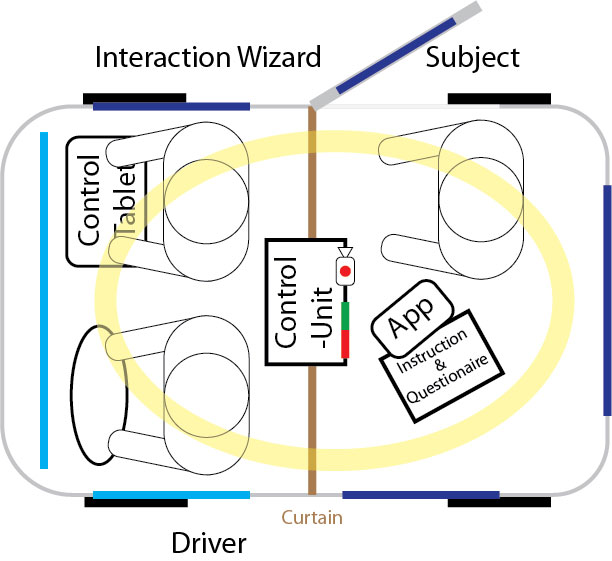
\includegraphics[width=0.7\textwidth]{fig/test-setup-hori}\hfill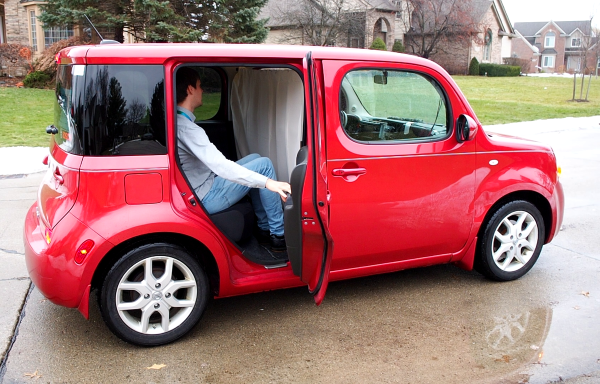
\includegraphics[width=\textwidth]{fig/enter.png}
    \caption[Driving Simulator]{Top: Seating of wizards and test subject. Bottom: Test subject entering the autonomous driving simulator}
    \label{fig:testsetup}
\end{figure}

A blackout curtain was attached between each sided of the B-pillar to separate the researcher from the passengers. It blocks shadows so that the silhouettes from the researchers are not visible. A light color and texture were used so that even though the curtain is right in front of the passengers, it does not feel close and oppressive. It was attached with a sturdy metal rope and needles so that it stays in place. The curtain was high enough that the heads of the driver and wizard could not be seen and low enough so that most people should be able to glance at the front of the light bar.  The control box was attached slightly above the curtain and cables were laid to the front and through the paneling to the battery. 

\subsection{Video Analysis}
\label{sec:videoAnalysis}
I recorded videos of the cabin as increasingly, it is being recognized that capturing behavioral data from participants, such as facial expressions or head movements, may be a more accurate representation of how and what they feel and a better alternative to self-report questionnaires that interrupt participant’s emotions and cognition during performance \citep[see][]{Ahn2011UsingPrediction}.

\begin{figure}
    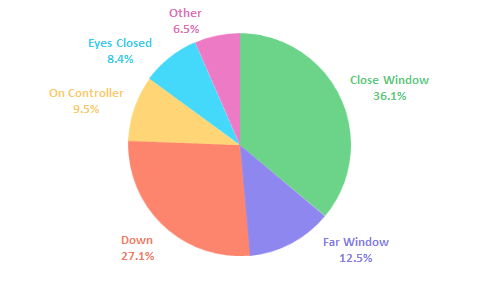
\includegraphics[width=0.5\textwidth]{fig/PieTotal.png}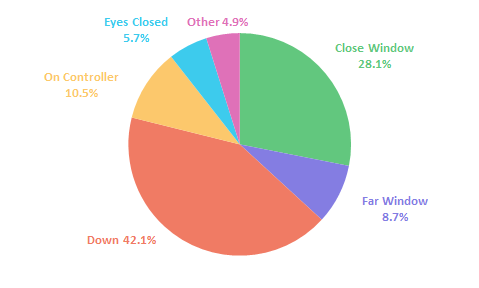
\includegraphics[width=0.5\textwidth]{fig/PieTotalNo.png}
    \caption[Total Times of Focus of Attention]{Total Times of Focus of Attention. Left: Guide On condition, Right: Guide Off condition}
    \label{fig:totalPie}
\end{figure}

The first impression of the participants when they enter the vehicle was that: five of them appear a little bit tired (yawning, sleepy eyes), five seem engaged (awake, looking out of the window, rereading the instructions), two skeptical (frown, contemptuous), one is relaxed (closing eyes), and one participant appears to be frightened (holding onto handrails). Participants shifted their attention constantly between inside the vehicle and outside the car; this is very different from drivers who have their eyes always on their road and the behaviour of relaxed passengers who are immersed in non-driving tasks. 
Three participants were listening to music or audiobooks on their own devices. Two participants were looking onto their smartphone for more extended periods (but less than 1/4 of the driving time), two participants tried to use their phone initially but stopped after a while, and three participants checked their phones briefly (for periods of a few seconds). One person closed their eyes for roughly 1/3 of the drives. 

We can see in the video how most of the participants used the information that was available to them: People checked the screen regularly and the light bar sparsely; Some people used the web app or opened Google maps to check their location; If they felt, heard or saw something they were checking the windows, the light bar, and the screen. As I did not track the location of the test car it is difficult to relate the events, messages and people's reactions with high precision, however, it appears that the typical chain of events was: participants head down - light message triggered - participant looks out of the window - event is executed in reality - participant checks the screen - the participant looks down again. 

No person used the 'Pull Over' button. A few people used the Light button to turn the light on to fill out the forms, and a few people turned the guide light off for a moment but turned it back on after having tried out the function. 

I analyzed half of the rides statistically as the light conditions allowed to see the subjects throughout both tours (n=7). The videos were coded with ELAN \citep{Wittenburg2006ELAN:Research}. Noticeable gestures and speech were written down. I categorized the direction of attention throughout the whole ride into the categories: Close Window, Far Window, Down, Far into Close Window, On Controller, Directly Onto Light Bar, Straight, Back, Eyes Closed (See \emph{\fullref{fig:videocode}}. These were combined into attention out of the vehicle (Windows), inside the vehicle (Down, Straight, Eyes Closed) and onto the Information (Controller, Light Bar). The individual events were averaged into duration's and normalized and summed into totals.
\begin{figure}
    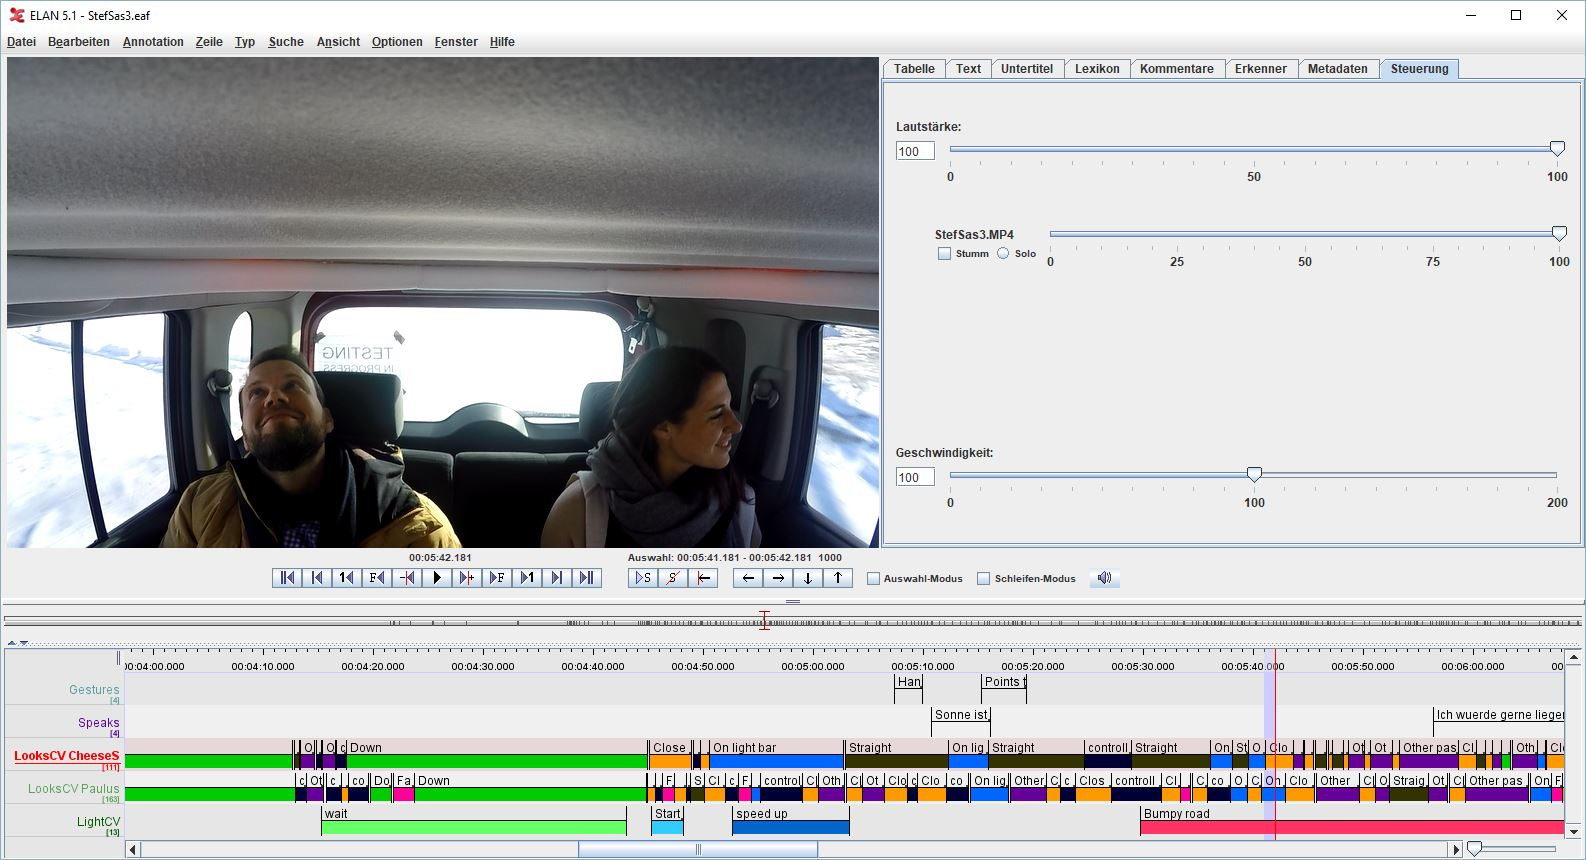
\includegraphics[width=1\textwidth]{fig/StefSas.JPG}
    \caption[Video Coding]{Video coded test ride}
    \label{fig:videocode}
\end{figure}
Since the data is approximately normally distributed (Shapiro-Wilk) ratio data, I used Paired Samples T-Tests to compare the times with guide on against guide off. In the 'guide on' condition, attention was marginally-significant\footnote{\url{https://www.psychologicalscience.org/publications/observer/obsonline/rise-in-reporting-p-values-as-marginally-significant.html}} longer outside the vehicle and significantly shorter inside the vehicle. These effects were all large (\emph{\fullref{tab:totalVideo}}). People were paying more attention to what was happening outside (\emph{\fullref{fig:attentionTotal}}); possibly they tried to consciously match what the messages indicated with what happened outside or the light directed their attention unconsciously back up. Thus, one might conclude that the light messages lead to more attentive rides. 

\begin{table}
\label{tab:totalVideo}
  \caption{Paired Samples T-Test of total time differences}
\begin{tabular}{@{}llllll@{}}
\toprule
 & statistic &  p & Mean diff. & SE diff. & Cohen's d \\ \midrule
Outside & 2.206 &  0.070 & 2.139 & 0.970 & 0.834 \\
Inside & -2.532 &  0.045 & -2.218 & 0.876 & -0.957 \\
Information & -0.050 &  0.962 & -0.028 & 0.572 & -0.019 \\ \bottomrule
\end{tabular}
\end{table}

\begin{figure}
    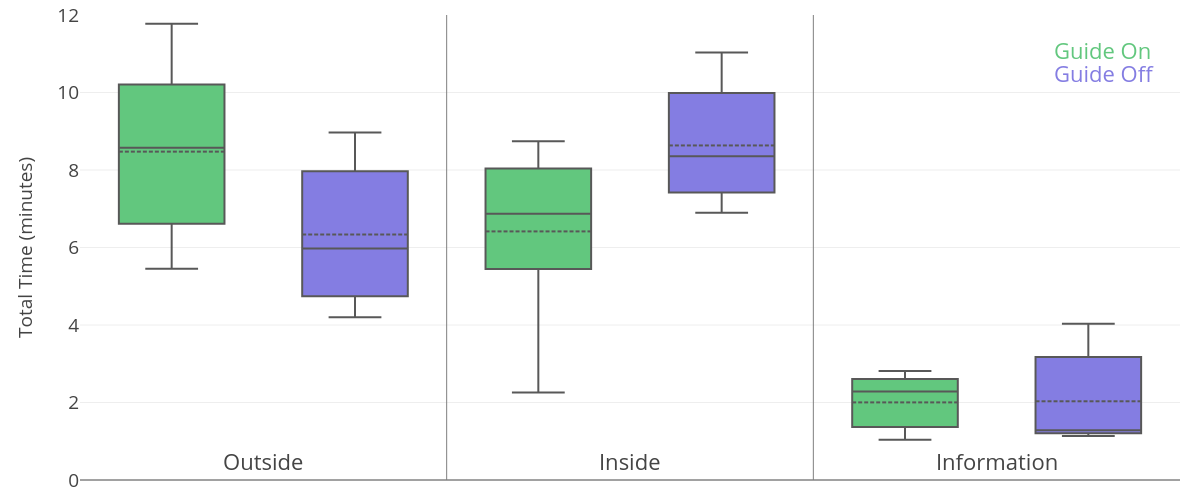
\includegraphics[width=1\textwidth]{fig/Total.png}\hfill\
    \caption[Times of Attention]{Total times of focus of attention}
    \label{fig:attentionTotal}
\end{figure}

The time that people looked at the information did not differ (p=.962, d=-0.0187), however we cannot say that the times are equivalent as a TOST \citep{Mara2012Paired-samplesEquivalence} Paired Samples T-Test shows
(TOST\textsubscript{Upper} t=-1.80, p-.061 ,and TOST\textsubscript{Lower}t=1.70, p=.070).
However, why did the total times' people checked the information did not differ? One possible explanation is that people expected something to happen, as they were part of an experiment, and therefore did not want to miss this event. Another theory is that people were reassuring themselves that everything is 'in order' by reading the message "Autopilot is active". Finally, it might be that participants were bored and looked onto the control display to 'rest their eyes'. These interpretations were reaffirmed by the interviews \emph{\fullref{ssec:interviews}}. 

\begin{table}
\label{tab:averageVideo}
  \caption{Paired Samples Wilcoxon W-Test of average duration differences}
\begin{tabular}{@{}llllll@{}}
\toprule
 & statistic & p & Mean diff. & SE diff. & Cohen's d \\ \midrule
Close window & 4.00 & 0.109 & -1.21 & 1.79 & -0.535 \\
Far window & 3.00 & 0.078 & -2.98 & 1.03 & -1.021 \\
Down & 2.00 & 0.047 & -7.06 & 1.91 & -1.327 \\
Looks straight & 15.00 & 0.402 & 1.09 & 1.37 & 0.310 \\
On control unit & 1.00 & 0.031 & -2.34 & 1.98 & -0.750 \\
On light bar & 7.00 & 0.297 & -2.86 & 1.85 & -0.548 \\ \bottomrule
\end{tabular}
\end{table}

\begin{figure}
    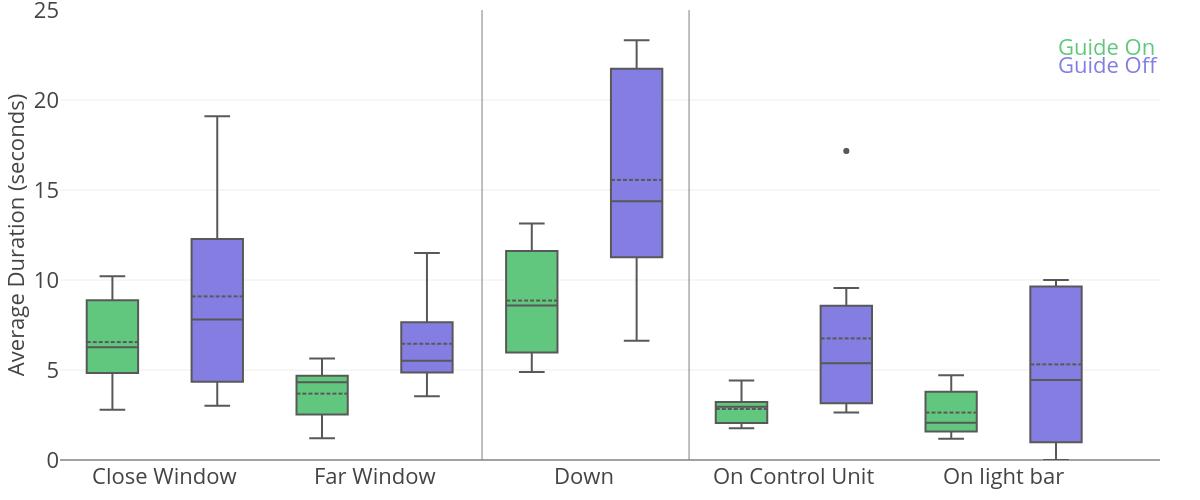
\includegraphics[width=1\textwidth]{fig/Average.png}\hfill\
    \caption[Average Duration of Attention]{Average duration of attention (For the complete statistical report refer to the digital appendix)}
    \label{fig:attentionAverage}
\end{figure}


In \emph{\fullref{fig:attentionAverage}} the average duration of focus of attention are shown. In 'Guide On' condition the passengers generally stayed shorter in one category of attention. Table \emph{\fullref{tab:averageVideo}} shows that for looking 'down' and looking 'on control unit' these differences were significant; for 'far window' the effect was marginally significant. These effect sizes were medium to large. Shorter dwelling in one spot shows more switches of attention conversely. As discussed in \emph{\fullref{ssec:carsickness}}, to look up and out of the window regularly can help against motion sickness. 

In summary: With the ambient light turned on passengers were spending less attention on their phones and focused more on the road. They were not spending more time monitoring the information from the ambient light, and they were riding more attentively. Looking out of the window regularly and during jerk could lower car sickness (see \citep{Eager2016BeyondDerivatives} for the use of terms acceleration, jerk and snap). The tours chosen for the test rides had many events (turns, speeding up and slowing down); on routes with more steady driving passengers, focus of attention might not differ in guide on and guide off conditions: the passengers can use their time for secondary tasks. 

\subsection{Questionnaire}
\label{ssec:questionaire}
Participants filled out the randomly ordered machine acceptance questionnaire two times (Guide On and Guide Off conditions). All questions (See  \emph{\fullref{tab:questionaire}}) were to be answered in the form of 7-point Likert Scales from 'not at all' to 'extremely'. The 'Scale of Trust in Automated Systems' is derived from \cite{Jian2010}. It asks participants to rank the car's behavior, to obtain trust and mistrust scores. Two attitudinal measures are taken from \cite{Koo2015}: annoyance (\say{How well do the following words describe how you felt while driving?"}) and assistance (\say{How well do the following adjectives describe the car?}). 

\newcolumntype{b}{X}
\newcolumntype{m}{>{\hsize=.7\hsize}X}
\newcolumntype{s}{>{\hsize=.45\hsize}X}
\newcolumntype{t}{>{\hsize=.1\hsize}X}

\begin{table}
  \caption{Questionnaire items and corresponding scores}
  \label{tab:questionaire}
\begin{tabularx}{\textwidth}{tmbss}
\toprule
& Trust
& Mistrust 
& Annoyance
& Assistance\\
\midrule
1. 
& \raggedright I am confident in the car
& The car is deceptive
& Anxious
& Intelligent\\
2. &  \raggedright  The car provides security& \raggedright The car behaves in an underhanded manner &    Annoyed    & Helpful
\\
3. &\raggedright The car has integrity& \raggedright   I am suspicious of the car's intent, actions or outputs&    Frustrated    &Dominant\\
4.&\raggedright The car is dependable&    I am wary of the car&&        Reliable
 \\
5. &\raggedright The car is reliable    & \raggedright The cars actions will have a harmful or injurious outcome&&
\\
6. &\raggedright I can trust the car &&&
\\
7.&\raggedright I am familiar with the car &&&
 \\
\bottomrule
\end{tabularx}
\end{table}

One strong outlier, who crossed multiple scales to the extreme values, was removed from the data (n=13). Scores were normally distributed according to Shapiro-Wilk tests and QQ-Plots. Composite scores were treated as ordinal data \cite{Boone2012AnalyzingData}, and Paired Samples T-Test were used to compare scores in the 'guide on' and 'guide off' conditions. Statistical analysis found no order effects for the scores on mistrust, trust, assistance and annoyance and no difference in reactions to route A and B. Mistrust increased slightly, but not significantly over time. 

\begin{figure}
    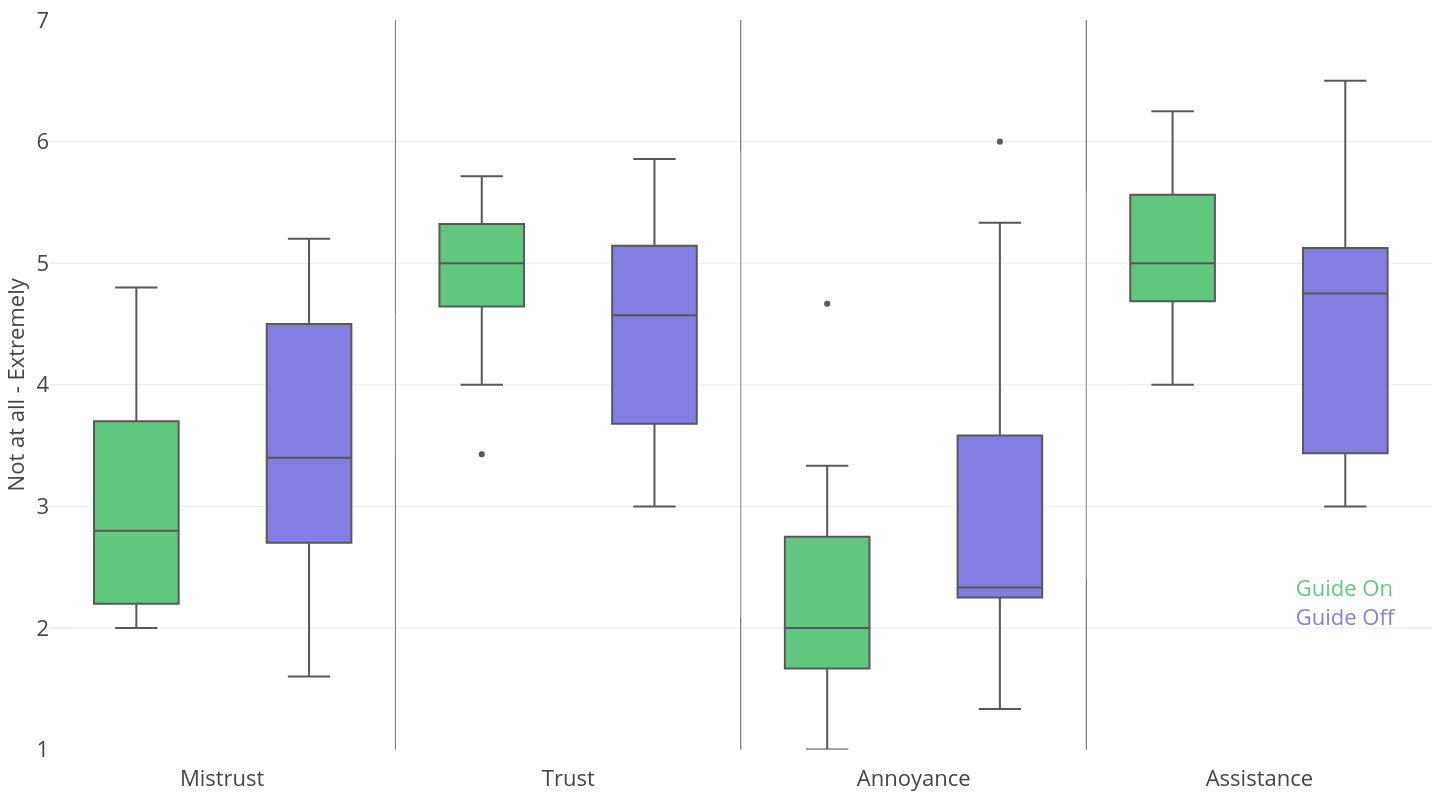
\includegraphics[width=1\textwidth]{fig/questionaire.png}\hfill\
    \caption[Scores from questionnaire]{Scores from questionnaire in conditions (For the complete statistical report refer to the digital appendix)}
    \label{fig:questionaire}
\end{figure}

There was no significant difference in trust and mistrust scores. Except for 'The car provides security' (W=54.5, p=.040, d=0.641) and 'The car is dependable' (W=31.0, p=.073, d=0.549) there was no significant or marginally significant differences in the Likert-Type questions that make up the composite trust and mistrust scores. Participants responses for 'The car is reliable', 'I am wary of the car' and 'The cars actions will have a harmful or injurious outcome' were equivalent (TOST Paired Samples T-Test: Cohen's d lower -0.5 and upper 0.5 equivalence bounds: p=.048).

One might interpret these results in the following ways: trust and mistrust establish themselves over a more extended period, trust is what people expect of the technology and comparable technologies after they have experienced it to work consistently safe (or not). In comparison, the ethnographic study by \cite{Lee2016} found that trust is positively influenced by feedback, but also found that social factors influence the attitudes towards trust in autonomous vehicles. Further, trust and mistrust are ill-defined measurements (compare how the cited studies in \emph{\fullref{sec:trust}} use all different measurements of trust). In addition, the interviews (\emph{\fullref{ssec:interviews}} revealed that people were too aware that the vehicle was not genuinely autonomous and who the driver was. Ultimately participants were trusting me to drive safely but (the researcher) to also create a safe test environment. When talking about trust, people thought of it more as a personality trait of themselves rather than of something they can see in a car. Finally, it might be that people knew that the driving style (or the driver) could not have changed between rides and therefore adjusted their responses: e.g., the reliability of the car and the likelihood of a fatal crash remain the same. In any case, it is worth to know that participants felt that the vehicle with feedforward information provided more security. % To imagine sitting in a fully self-driving vehicle is unimaginable for most people

There was a significant difference (two-tailed, p<0.05) in scores for annoyance (t=-2.293, p=.041) in the 'guide on' (M=2.308, SD=0.957) and 'guide off' (M=3.026, SD=1.536) conditions. 
The assistance score was significantly different (t=2.987, p=.011) between 'guide on' (M=5.135, SD=0.650) and 'guide off' (M=4.462, SD=1.111) conditions. The change in annoyance has a medium effect size (d=-0.636), and change in assistance has a large effect (d=0.828). Participants experienced the vehicle with ambient light as strongly significant more helpful (W=55.0, p=.006, d=1.239) and significantly more intelligent (W=26.0, p=.049, d=0.660). The outcome of the assistance score is somewhat expected. Of course, a vehicle that gives feedback and explains what it is doing is more helpful and more intelligent than one that does not. The improvement in the annoyance score is promising as it is not self-evident. It is quite possible that people would be annoyed by the light feedback, as it is common with sound feedback. Moreover, it might be that they feel more frustrated as it could make them aware of situations which they can not influence either way. Finally, some test subjects (the outlier too) were close to being extremely frustrated with their situation in the back of the vehicle: Everything that helps people to feel more comfortable is worth to look into. 

% Effect size was calculated as normal approximation of z to r \cite{Wuensch2015NonparametricSize}; We observed a medium change in annoyance (r = 0.401) and assistance (r = 0.471). No effect could be found of conditions on trust or mistrust.

%Diagrams of trust etc.
\subsection{Follow up questionaire}
In Table \emph{\fullref{tab:order}} the light messages are ordered by their perceived helpfulness. People liked to be warned of the jerk (brake, swerve and acceleration) but also of conceptual states (Start/ arrive destination, Wait for traffic light). People liked events that they could perceive simultaneously by other modes less: 'speed up' could be noticed by the motor sound and 'Turn left/ right' could be heard by the sound of the blinker and seen by the lane in which the vehicle joined. 'Enter /Exit' highway was ranked low because it only occurred once. Only a few rides had the event 'drive backward' (when the vehicle had to move backward because a vehicle parked in front of it), but it was well received by those who did: \begin{quotation}\emph{Move backward was really good. That the vehicle told me that, because I did not expect it to go backward}\end{quotation} As we described in \emph{\fullref{ssec:questionaire}}, participants did not use the light messages to establish trust in the 'autonomous vehicle' in this study; but they liked to be informed of those events nonetheless. 

\begin{table}
  \caption{Light Messages Ordered by Helpfulness}
  \label{tab:order}
  \begin{tabular}[t]{clcc}
    \toprule
    Order & Message & Mean & Std. Dev.\\
    \midrule
1.  & Brake intensity                     & 2.3 & 1.1 \\
2.  & Start / arrive  at destination       & 2.6 & 1.7 \\
3.  & Start moving (drive off)            & 3.6 & 2.7 \\
4.  & Swerve (obstacle)                   & 3.9 & 2.3 \\
5.  & Wait: traffic light / pedestrian & 4.0 & 2.5 \\
6.  & Move backwards                      & 4.1 & 3.0 \\
7.  & Bumpy  / slippery road               & 4.4 & 2.6 \\
8.  & Change lane                         & 4.6 & 3.0 \\
9.  & Speed up / slow down                & 4.7 & 3.1 \\
10. & Turn left / right                   & 4.9 & 3.1 \\
11. & Enter / Exit highway                & 6.4 & 2.9
\end{tabular}
\end{table}

To the question 'If you are a passenger in an autonomous vehicle, which information do you need during the ride in order to feel comfortable ?' 
\textbf{86\%} replied 'Trip progress information' (Time to arrival, detours), \textbf{78\%} wanted 'Feedforward decision information'(What is the car about to do soon, e.g., start moving), \textbf{64\%} wanted this type of information only for exceptional events (e.g., strong brakes), \textbf{50\%} wanted to see sensor data, and \textbf{42\%} wanted to know 'Feedforward reasoning information' (Why is the car about to do this? E.g. possible passenger on road detected: slow down). In 'Car engine parameters'(Mph, acceleration force, engine temperature, gear) \textbf{35\%} were interested, in the 'Recognition state'(E.g., Which other cars are recognized at the moment) \textbf{28\%} and in 'Feedback information'(E.g., why did the car slow down) \textbf{28\%}. One person mentioned that he needs to know the 'Fuel/Battery information' and one person stated that he needs the 'Position on a map'. No person stated to need no information in order to feel comfortable. 

\textbf{21\%} of people stated that knowing what was about to happen made them feel 'extremely' more comfortable. \textbf{64.3\%} closer to extremely (4 in a 5-point Likert-Type scale). \textbf{One} person crossed the undecided centre and \textbf{one} closer to 'not at all' (M=4.00, SD=0.78). \textbf{87\%} could comprehend what the lights were indicating and \textbf{21\%} not. \textbf{64\%} could comprehend what the vehicle was doing next and \textbf{35\%} not. People had a slight positive tendency for 'Is text an appropriate mode to convey what the car is about to do?' (M=3.5, SD=1.40) and  'Is light and appropriate mode to convey what the car is about to do?' (M=3.5, SD=1.09). This can also be found in the replies to 'Would another modality have worked better for this type of driving information': Icons on a screen (\textbf{50\%}), Light is good (\textbf{35\%}), Sound (\textbf{35\%}), Voice (\textbf{21\%}), Light only (\textbf{14\%}) and Text only (\textbf{0\%}). 

These results show that participants were enjoying the concept of feedforward information in autonomous vehicles but saw some need to improve the communication. Indeed the reflective strength of the light messages was weakened (\emph{\fullref{sec:limitations}}), a screen directly in front of the passengers would not have any visibility issues (\emph{\fullref{fig:fig-waymo}}). In the \emph{\ref{ssec:interviews}} some people voiced strong aversion to sound and speech: 'annoying beeps', 'stupid robot voice' and 'subway announcements'. 

\subsection{Interviews}
\label{ssec:interviews}

I transcribed and coded responses from all interviews (n=14). The most frequently mentioned topics were (in descending order): windows, direction of attention, feedback and driving style. In the following, commonly discussed topics are grouped(a few < 4, some 4-6, several 7-10, most > 10): Most participants thought it was necessary to have a good overview of road conditions at all times, they did not want to sit in a windowless cabin or be seated backward. They disliked being seated in the back seat, not able to look out through the front. Only a few participants thought they would be able to recline and sleep in such a vehicle. These people also mentioned that a restricted view would further free them from responsibility. Some participants had issues experiencing the ambient display in peripheral sight because of the bright light conditions outside ( \emph{\fullref{sec:limitations}}). Several participants mentioned how the light guided their attention. Several participants said the light did not annoy them, and that they would want it to be always on. Several voiced they would not want to have sounds, whereas a few wanted to have an escalation stage with sound warnings. A few wanted to be able to customize light intensity or which light messages show up (e.g., disable information about turn taking).

\begin{quotation}\emph{... And then I realized that I do not want to read that much up there. Once you have seen all the commands, then the light is enough even without text. Then the light is more interesting}\end{quotation}
Most participants stated that driving style would have the highest influence on their comfort and that they would want the cab to drive very smoothly. Only a few wanted the vehicle to drive faster, e.g., in situations of urgency. All participants enjoyed being informed about acceleration changes.
\begin{quotation}\emph{The car does what it wants to do anyway, but at least it tells me what it does.}\end{quotation}
A few participants felt irritated when the vehicle did not announce upcoming bends as they expected this from the turns. On the other hand, some participants said to display vehicle actions which can be perceived via other modalities would be unnecessary (e.g., one can hear the blinker, see in which lane the vehicle moves, or hear the motor when the car accelerates). All participants talked about the learning process for the light messages: Most stated that they initially looked at the display but stopped paying attention because the light was enough information. One person said the display was distracting because he would look at it rather than at his phone. Some people wanted the light messages to be displayed even earlier. \begin{quotation}\emph{
With the light one feels much more comfortable, that is extremely important}\end{quotation}
Several people talked about how they establish trust over longer time periods whereas a few mentioned that they would be very trusting right from the start. One person stated to have extreme car sickness and that the driving was extremely uncomfortable for them because of that. This person believed that all driving information enables anticipating what will happen and therefore can help against driving sickness. 

\subsection{Limitations}
\label{sec:limitations}
Participants might have compared between both conditions and abstracted their responses to these questions. Possibly, an independent study design would have yielded different results.

One of the most significant issues with the study was the very bright lighting conditions outside. The test drives were conducted in January 2018 in Detroit, Michigan with more than 10cm snow. The test drives were taking place shortly after the lunch break not to take too much time from the employees: The sun was intense and because of winter times quite low; Light was shining directly into the cabin and also reflected from the snow towards the ceiling of the car where the light ring is situated. The driver even had to wear sunglasses to protect against the bright sun. However, the \emph{\fullref{sec:videoAnalysis}} revealed that people did react to the light messages: Possibly they did not register all light messages consciously but only were made aware of a change subconsciously. 

People were on their own during the study (\emph{\fullref{sec:study}}), they were separated from the researcher and instructed to call a number or press the 'stop' button in case of an emergency. However, people knew that the vehicle did not drive itself, as they were colleagues of the researcher, and they also knew that most likely I was driving the vehicle. Interestingly, no person was aware that a second person was seated in front to control the light messages. Technological less savvy participants could have taken the wizard cab as an autonomous vehicle, and undoubtedly external test subjects could have more mistrust in the researcher.

Besides, the light messages were controlled by the interaction wizard ( \emph{\fullref{sec:wizard}}), even though he was trained the light messages sometimes were triggered inconsistently. People might make more use out of the light messages if they align routinely to the driving behavior. Some people mentioned that they wanted the light messages to trigger earlier ( \emph{\fullref{sec:interfaces}}). 

Finally, the participants were acquainted with the researcher and maybe tried to reply to his expectations, even if they were told not to do so. 

\section{Workshops}
I was already early on attempting to find participants for a participatory design workshop as it was recommended by \cite{Pettersson}. I put up flyers in local libraries and supermarkets. As I was looking for people with limited mobility I was in contact with 'meals on wheels' Area Agency on Aging 1-B\footnote{https://aaa1b.org/} who were highly positive about requiring people for our common goals. After many attempts to find a possibility to bring the interested people together in one place, I parted with the idea to hold a workshop. In hindsight, it was a doomed idea to hold a workshop with restricted mobility people in an area where the whole infrastructure is car-based. Even though Bosch agreed to pay for fuel and catering it was not possible to pick up all individuals scattered in a radius of up to 17 miles. The lesson learned is that in particular car-based cities and communities without the prospect of improvements in public transport options could benefit the most of autonomous vehicles. 

Back in Germany, it was easier to find people for two workshops ( \emph{\fullref{fig:workshop}}). The opinion of people with restricted mobility about autonomous vehicles and the light interface was investigated. I held the first workshop at an assisted living center (DRK Service-Wohnen 2, Weimar). One male and nine female seniors in the ages from 67 to 95 participated. For the second workshop, three mobility restricted participants (one 41-year-old male and two females aged 45 and 46) were recruited from counseling (Lebenshilfe-Werk Weimar/Apolda e.V.), and a social work student drove them to the university where the workshop took place. 

Both workshops started with a brief introduction of each participant and their difficulties and limitations in day-to-day life. Then we discussed the pros and cons of autonomous driving. Next, each participant picked a destination they cannot or choose not to go often. Then, we used printed maps of tours to illustrative locations (e.g., doctors and sights) to discuss their difficulties with public transport and taxis. Later on, photos of potential autonomous vehicles (private and public), as well as current prototypes (Waymo, Olli), were shown. In the first workshop, a video where a Youtuber\footnote{\url{https://www.youtube.com/watch?v=oRUq3TBj7yM}} explained the technical function of autonomous vehicles was played back. This video was ill-received, thus in the second workshop I showed videos of the Waymo self-driving vehicle instead \footnote{\url{https://www.youtube.com/watch?v=B8R148hFxPw}}\fnsep\footnote{\url{https://www.youtube.com/watch?v=aaOB-ErYq6Y}}  and explained some operating principles myself. We used the maps from earlier and the demonstrator (Fig: \emph{\fullref{fig:demonstrator}}) to discuss and design their ideal self-driving vehicle. Then, I showed them the light messages from the prototype and where they would trigger along the exemplary routes. We used the live interface ( \emph{\fullref{fig:liveinterface}}) to discuss, create and fine-tune light messages. Lastly, an amusing video about backseat driver behavior was shown \footnote{\url{https://www.youtube.com/watch?v=CeWQCLJCLSg}}. 

\subsection{Workshop 1: Seniors}
\begin{figure}
    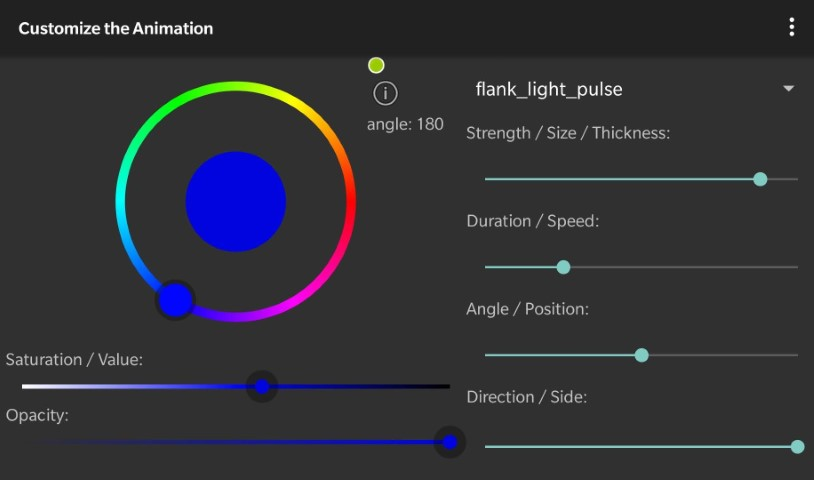
\includegraphics[width=0.9\textwidth]{fig/customAniShrunk.jpg}
    \caption[Light mixing interface]{Interface to mix custom light messages}
    \label{fig:liveinterface}
\end{figure}
\begin{figure}
    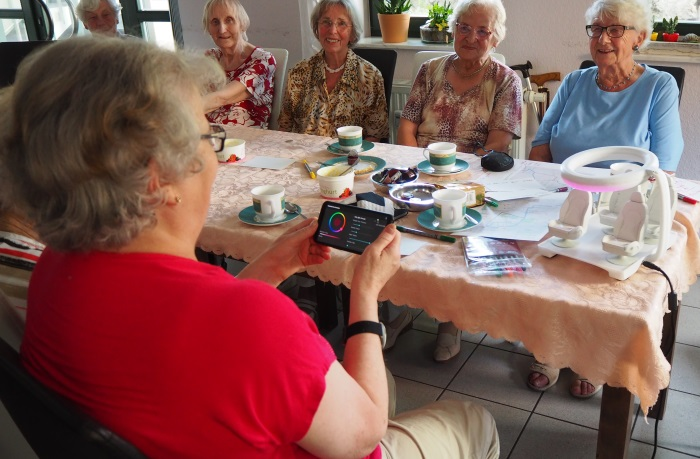
\includegraphics[height=0.3\textwidth]{fig/omis.jpg}\hfill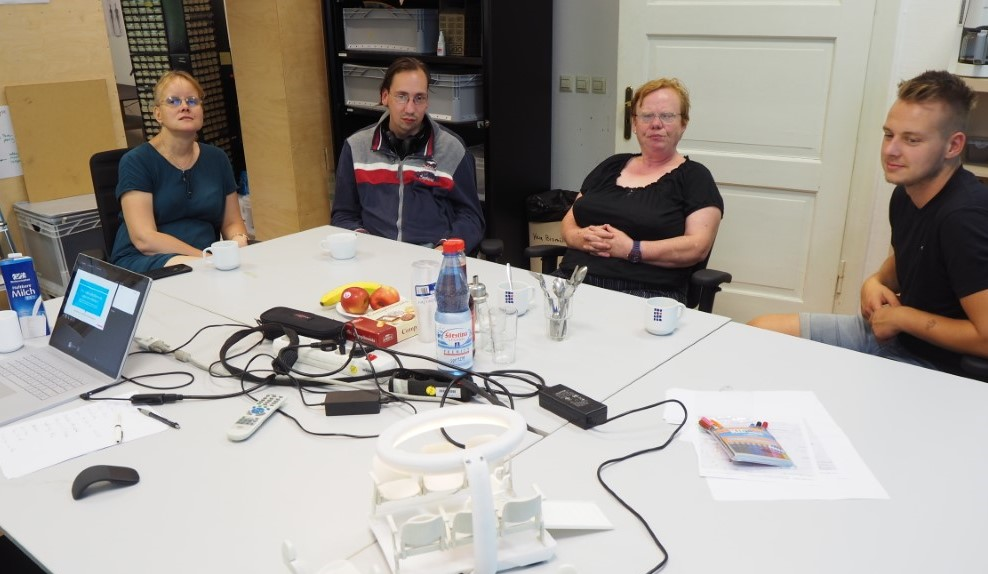
\includegraphics[height=0.3\textwidth]{fig/workshop2.JPG}
    \caption[Workshop]{Left: Workshop 1 participant using the live interface. Right: Workshop 2}
    \label{fig:workshop}
\end{figure}
The seniors were impressed by the technology of self-driving vehicles and the demonstrator but skeptical of the impact of self-driving vehicles. In particular, they were concerned about the loss of human contact because of automation and the necessity to develop self-driving vehicles. After we discussed the pros and cons some of the participants mentioned that their skepticism might be grounded in their age \say{I am happy that I can use my iPad}, \say{I would never enter a plane, but my daughter flies all the time}. 
Furthermore, they agreed that a lot of older adults are isolated precisely because of their immobility and that they would fare better than others because of their shared living community. Most seniors pointed out that they leave their community very rarely: They have their doctors come by, eat together in the in-house canteen, order food and clothes by phone and some even online and have their families visit. Further mentioned reasons were that with age they lost their interest to go somewhere else, had difficulties with public transport and could not afford taxis. The public transport around them is as it happens affordable, close and frequent (Bus stop is located right at the communities door), yet most of them use it less than once a month. The seniors emphasized multiple times how difficult it is to use the bus at their age: \say{I feel rushed because the driver has to follow his schedule and I need too much time to sit down}, \say{If there are no seats I do not want to be the old person who asks other people to stand up}, \say{The entrance door is too high}, \say{Once I fell over, because the bus started to drive abruptly, and since then I have not used the bus}, \say{There is no place to put my walker}. The seniors once participated in a workshop 'Gain the confidence to drive the bus' but bus usage has not increased much. They preferred the train but said that they do not use it because of the difficulties to get to the train station by bus first. 
The participants would want to use an autonomous vehicle (if they dare to use it or a cheap Taxi) to go to the doctor, to go to shopping centers, to visit friends and to go on vacation with distances ranging from 3km to 200km.  
The seniors mentioned that there should be different versions of vehicles for different needs and that they would need a vehicle equipped for the disabled (with a ramp, comfortable seats, and handrails). The seniors liked the interface, in particular, to start and stop the vehicle by themselves and the light signals to know when they need to hold onto rails. However, they could not imagine whether it will help them to feel comfortable and said that they would have to experience it for themselves. They would like to see a map inside the vehicle itself so that they know that the vehicle is driving where they want it to drive to, and have some sound feedback, too. They do not want to have to read text or listen to a voice. They would want to order the cab by a phone call or have relatives call them. Moreover, they liked the idea to have somebody (e.g., the relatives they are driving too) on a screen to chat with. 


\subsection{Workshop 2: Mentally and physically impaired people}
The participants in this workshop were highly interested in self-driving vehicles. They were mostly concerned about the price and safety of such a car but would want to own such a vehicle for themselves. They mentioned that they would not want to share it with others because of the cleanliness. It would help them to get to their (supervised) work and family in other cities. One participant said that she would want to have it drive slowly so that she can read during the ride. The participants said that their comfort (in cars and taxis) mostly depends on the driver. All of the participants are capable of using the bus and sometimes use it. One woman who has issues with her legs mentioned a scenario where she could not sit because even the disability seats were taken. The people who occupied the seats did not get up despite her showing the Disabled ID card and the bus driver refused solve the situation as he is 'just the driver'. Other than that they mentioned that people usually give space if they ask directly. Many people have issues with entering, exiting and sitting down in buses, trams, and trains but the drivers usually do not help. It would be good to have somebody help to enter and exit. The participants thought that the light interface is a good idea but said that blind people would want to know the same information too; they cannot locate themselves. The light animations should be standardized: \say{This light should be standardized as road signs are}. People would need to learn them only once. However, some young people would want the choice to set the color of the car themselves. They thought red colors for braking, yellow colors for turns were a good choice but they would change the blue color for 'start moving' to green.  They thought a voice would be distracting and that a screen would keep them from reading or watching the scenery. Finally, they wanted additional information for hardware and software faults of the vehicle and wanted to be able to directly ask the vehicle for information about sights that they can see through the window.
